\section{Tracks and datasets}
\label{sec:tracks}
\begin{table*}[t]
    %\hspace*{-1.5cm}
    \footnotesize
    \begin{tabular*}{\textwidth}{c|ccccccc}
        \toprule
        Track    &  Dataset  &  Datatype  & Dim. & Distance & \#Vectors  & \#Queries & Terms \\
        \midrule
        {Filtered}  & YFCC    &  uint8     &    192      &    $\ell_2$   &    10M   &   100K     &  CC BY 4.0  \\
        {OOD}       & Yandex T2I &  float32  &    200      &    IP   &    10M    &   100K     & CC BY 4.0 \\
         {Sparse}   & MSMARCO/SPLADE    &  float32     &  <$10^5$  &     IP     &   8.8M  &    7K   &   CC BY 4.0      \\
        {Streaming} & MS Turing &  float32    &    100      &    $\ell_2$   &    N/A   &   N/A     &  \href{https://big-ann-benchmarks.com/MSFT-Turing-ANNS-terms.txt}{link}  \\ 
        \bottomrule
    \end{tabular*}
~~
    \caption{Overview of datasets used for each of the four tracks, their sizes, dimensions, and other properties.}
    \label{tab:data_details}
    \vspace{-15pt}
\end{table*}

The competition consisted of four tracks.
%
In each track, the entry must construct an \emph{index} from a \emph{database} of vectors or dense representations
of objects, optimized for the variant of queries applicable to the track.
%
Participants could submit separate entries to one or more of the tracks.
%
Each track uses one dataset listed in Table~\ref{tab:data_details}, which also summarizes their properties. 
%
All the datasets\footnote{All data was collected in compliance with the user agreement of a product or service,
and in the case of the MSMARCO dataset, with the consent of crowdsourced editors.} are available for
download from public cloud storage accounts without registration.
%
Except in the case of the streaming track, each dataset consists  a set of dataset vectors that
are supposed to be indexed, and a set of query vectors.
%
The dataset was made public during the development phase of the competition. 
%
For the final evaluation, the dataset vectors remained fixed, while a fresh set of query vectors, unseen to participants, was used.
%
Each track was evaluated independently with its own leader board.


%\magdalen{I added footnotes on data collection and on content of datasets to comply with the checklist.
%NeurIPS asks that we mention whether datasets contain identifying information and offensive content.}

\begin{figure*} 
\centering
\small
\begin{tabular}{ccc}
\bf Query & 
\multicolumn{2}{c}{\bf Database} \\
\raisebox{-0.5\height}{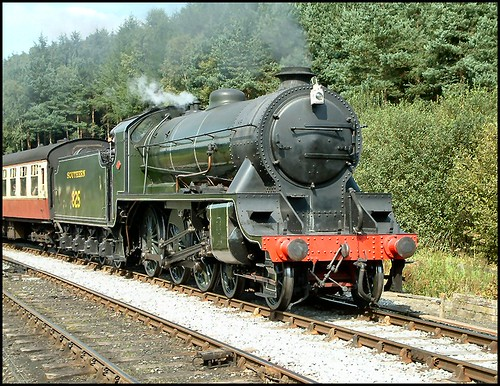
\includegraphics[width=3cm]{fig/226264627_90d8eaeb1f.jpg}} & 
\raisebox{-0.5\height}{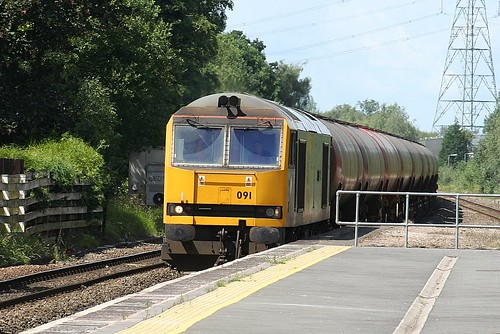
\includegraphics[width=3.5cm]{fig/755174504_7a9eee2248.jpg}} & 
\raisebox{-0.5\height}{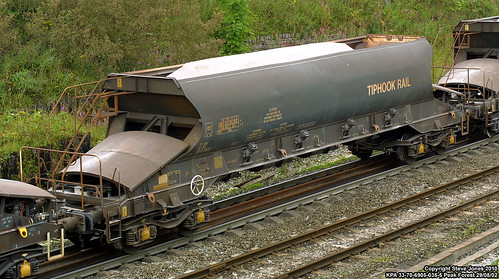
\includegraphics[width=3cm]{fig/5174840406_01fb734503.jpg}} \\ 
\\
\framebox{
\begin{minipage}[t]{3.7cm}
\footnotesize
freight \\ country\_GB
\end{minipage}
}
& 
\framebox{
\begin{minipage}[t]{4.7cm}
\footnotesize\flushleft
year\_2007	month\_July	camera\_Canon \textbf{country\_GB}	ukrail	tankers	
%Martin: edited out to make example a bit shorter
%loco	orton	tanks	workhorse	trainspotting	johngreyturner	
horsepower	haul	britishrail	rail	locomotive	diesel	machine	railway	british	\textbf{freight}	work	power
\end{minipage}
}
& 
\framebox{
\begin{minipage}[t]{3.7cm}
\footnotesize\flushleft
camera\_Canon	\textbf{country\_GB}	kpa	derbyshire	transport	rolling	rail	peak	wagon	britain	stock	railway	british	\textbf{freight}	forest	train	
\end{minipage}
}
\end{tabular}
\caption{
\label{fig:yfcc}
    Example images from the {Filtered} track, and  their associated tags: query (left) and database (right).  
    The images are represented by CLIP embedding vectors. 
}
\vspace{-7pt}
\end{figure*} 


\subsection{Filtered Search Track}
Searching for entities using a mixture of their semantic properties and associated keywords is natural and pervasive.
%
A couple of examples include searching for a visual match for an image, but from a region or associated with a certain kind of license,
or querying articles on arXiv based both on semantic match and time range or author affiliation.
%
This track explored how to build indices that optimize for such queries.
%
This task used the YFCC 100M dataset~\cite{thomee2016yfcc100m}, which consists of embeddings of images from Flickr\footnote{Flickr's content policy prohibits offensive images and images that contain identifying information.}. 
%
We used 10M random images from YFCC100M and embedded them using CLIP embeddings~\cite{radford2021learning}.
%
In addition, we associated to each image a ``bag of tags'': words extracted from the description, 
the camera model, the year the picture was taken, and the country.
%
This data was encoded as a sparse vector in the dataset.
%
See Figure~\ref{fig:yfcc} for an illustration of datasets and associated tags. 
%
The tags are from a vocabulary of 200,386 possible tags. 
%
The 100,000 queries consisted of one image embedding and one or two tags.
%
The index returns the images from the database with closest embeddings such that each 
image's ``bag of tags'' \emph{must}  contain all of the query's tags.

\subsection{Out-Of-Distribution Track}
This track modeled the scenario where the database and query vectors have different distributions in the shared vector space.
%
As observed in~\cite{jaiswal2022ooddiskann}, existing ANN search indices provide limited recall on such datasets.
%
This track used one such data set -- the cross-modal Yandex Text-to-Image 10M.
%
The database is a 10M subset of the Yandex visual search database
\footnote{The Yandex visual search database removes content where required by law. We were not able to determine whether the dataset creators further restricted identifying or offensive information from the dataset.}
represented by  200-dimensional image embeddings produced by the Se-ResNext-101 model~\cite{hu2018squeeze}.
%
The query embeddings corresponded to the user-specified textual search queries and were extracted with a variant of the DSSM model~\cite{huang2013learning}.\footnote{This dataset is a point in time and we do not have access to underlying data.}

A simple PCA projection of a sample of query vs. database vectors already shows the discrepancy of distributions.
Figure~\ref{fig:pcaOOD} shows the effect of out-of-distribution data. 
For illustration, let's look at the low-dimensional data, ignoring it’s a projection. 
The left plot shows that many text queries (in the lower-left side of the plot)
have the same database nearest neighbor because the database cloud of points does not reach so far to the lower left. 
This means that the optimal index should be more accurate (or have higher resolution)
on part of image database distribution that is most likely to be returned. 
Similarly, the right plot shows that many database images (in the lower right) will never be returned as the nearest neighbor of a query because they are in an area of the space where there are no queries. 
This means that an optimal index would just ignore these points altogether. 
We refer to~\cite{jaiswal2022ooddiskann} for characterizations of distribution mismatch for vectors and thus OOD results.

\begin{figure*}
% generated with https://github.com/harsha-simhadri/big-ann-benchmarks/blob/mdouze/additional_analysis_rebuttal/notebooks/visualize_OOD.ipynb
    \centering
    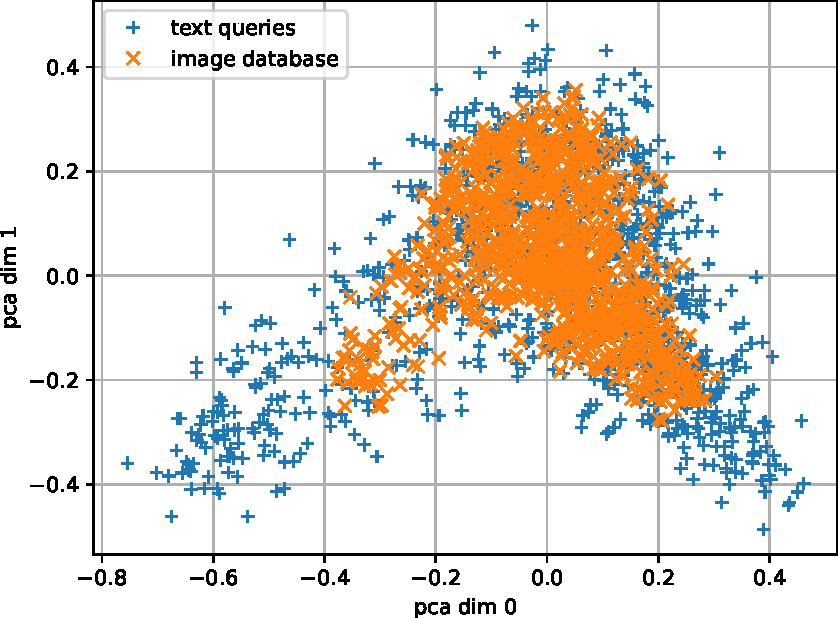
\includegraphics[width=0.45\linewidth]{fig/PCA_OOD_dim0_1.pdf}
    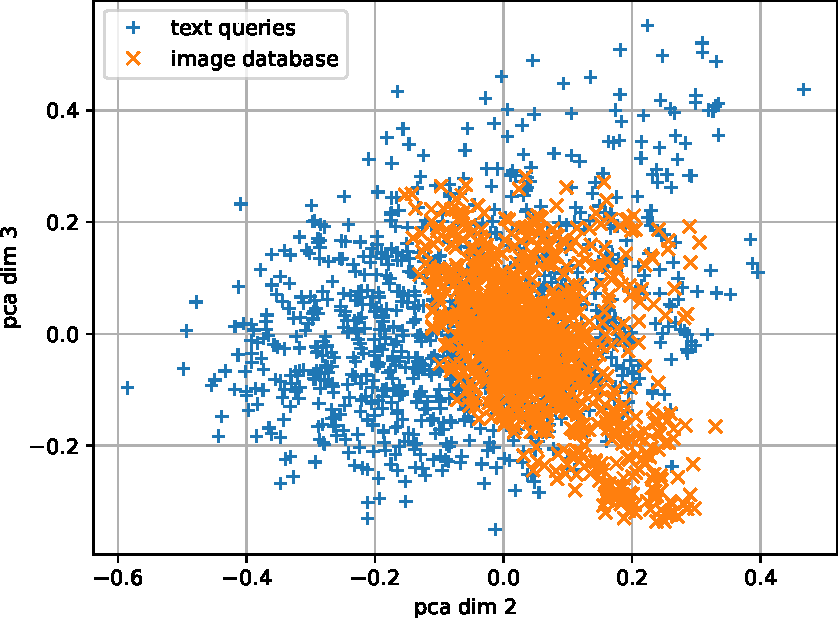
\includegraphics[width=0.45\linewidth]{fig/PCA_OOD_dim2_3.pdf}
    \caption{
    PCA projection of 1000 arbitrary query vectors and 1000 database vectors from the OOD dataset. 
    Left: the two first PCA dimensions, right: the two following ones.     
    }
    \label{fig:pcaOOD}
    \vspace{-.7pt}
\end{figure*}


\subsection{Sparse Track}

This task was based on the common MSMARCO passage retrieval dataset \cite{nguyen2016msmarco}, which has 8,841,823 text passages\footnote{The passages are anonymized and thus do not contain identifying information, but we were unable to determine whether offensive content was otherwise excluded.}, encoded into sparse vectors using the SPLADE model~\cite{formal2022splade}. The vectors have a large dimension (less than 100,000), but each vector in the base dataset has an average of approximately 120 nonzero elements. The query set was comprised of 6,980 text queries, embedded by the same SPLADE model. The average number of nonzero elements in the query set is approximately 49 (since text queries are generally shorter). 
Given a sparse query vector, the index should return the top $k$ results according to the maximal inner product between the vectors.


\subsection{Streaming Track}
In this track, the underlying databases evolved over time, and participants were to design an index
that supports insertions, deletions and searches.
%
While in practice such indices must support concurrent operations, we allow the index
to batch process one class of operations at a time for simplicity.
%
The index starts with zero points and must implement a ``runbook''  -- a sequence of batches of insertion operations,
 deletion operations, and search commands in a ratio of roughly 4:4:1.
%
This task used a 10 million vector slice of the MS Turing data set released in the previous challenge\footnote{The MS Turing dataset consists of Bing queries and answers.
We were not able to determine if it explicitly excludes offensive content and identifying information.}~\cite{DBLP:conf/nips/SimhadriWADBBCH21}.
%
 In the final run, we used a different runbook than the initial release to avoid participants over-fitting to the runbook.
% 
The \href{https://github.com/harsha-simhadri/big-ann-benchmarks/blob/v0.3.0/neurips23/streaming/final_runbook.yaml}{final runbook} consists
of 1280 batches of operations consisting of 5 rounds. 
%
To \href{https://github.com/harsha-simhadri/big-ann-benchmarks/blob/v0.3.0/neurips23/streaming/final_runbook_gen.py}{generate this},
we clustered the 10M points into 64 clusters.
%
Each round consisted of $4\times 64 = 256$ steps: insert a sample of points from a cluster, search the index using all the queries,
delete a fraction of points in the cluster, and search the index again.
%
This simulates distribution draft and point expiration which are both patterns is real workloads.
%
We enforced a memory limit of 8GB to ensure that indices were eliminating the data from the index and a time bound of 1 hour to carry out the whole runbook.

